\chapter[From Muscle Forces to Joint Torques]{From Muscle Forces\\to Joint Torques}
\label{ch:muscle-to-torque}
\raggedbottom
\index{moment arm}

\begin{laymansbox}{The Bridge Between Anatomy and Physics}{context:muscle-torque-bridge}
A muscle pulls on a changing anatomical path. That pull can turn several joints, resist their motion, or transmit power between them. The same net joint torque can arise from different muscle forces. This chapter connects those observations through geometry, virtual work and force limits, then asks what they let us infer about a golf swing. The numerical examples are constructed teaching cases, not measurements of a golfer.
\end{laymansbox}

\section{The Problem: Muscles Pull, Joints Rotate}
\label{sec:muscle-torque-problem}

A skeletal muscle contains fibers with different orientations and internal structures. A tractable musculoskeletal model often represents a muscle-tendon unit by one or more tensile paths. A compartment's transmitted tendon tension $F_j\geq0$ acts along its modeled path; it is not automatically the force of every fiber in the anatomical muscle. Fiber force, pennation, tendon compliance and activation dynamics determine how that tension develops. The muscle-force-generation chapter treats those physiological steps.

Here the immediate question is geometric: given a configuration and a set of path tensions, what generalized forces do they exert on the skeleton? We use independent coordinates $\bm q$, increasing path length $\ell_j$ to mean lengthening, and positive tension to mean pulling. These conventions fix the signs of torque and power. A torque is not itself a rotation: acceleration also depends on inertia, other forces and constraints.

For the initial derivation, paths are massless and frictionless, carry uniform tension, and depend only on configuration. Their routing constraints do no additional work. Moving guides, friction, path inertia and independently prescribed attachment motion require additional force or power terms. Declaring this boundary is part of the model, not an anatomical assertion about every tissue.

\section{Moment Arms and the Geometry of Force}
\label{sec:moment-arms}

\subsection{The Basic Definition}

Let $\bm\rho$ be a position vector from a point on a fixed rotation axis to a force application point, let $\bm e$ be the axis unit vector, and let $\bm f=F\bm d$ with $\|\bm d\|=1$. The moment vector and its signed axial component are
\[
\bm m=\bm\rho\times\bm f,\qquad
\tau_e=\bm e\cdot\bm m=F r_e,\qquad
r_e=\bm e\cdot(\bm\rho\times\bm d).
\]
The scalar $r_e$ has units of length and can be positive, negative or zero. Changing the reference point along the same axis leaves $\tau_e$ unchanged. Reversing the positive axis reverses both $r_e$ and $\tau_e$.

\begin{definition}{Moment Arm}{moment-arm}
A signed moment arm is the torque about a specified positive rotational coordinate per unit positive tensile force. For a single rigid rotation and point force it is $r_e=\bm e\cdot(\bm\rho\times\bm d)$. In a planar problem its magnitude is the perpendicular distance from the pivot to the force line. In three dimensions, distance from a force line to an axis alone does not determine the axial torque; force direction and axis projection matter.
\end{definition}

The magnitude $\|\bm m\|=\|\bm\rho\|F\sin\alpha$, where $\alpha$ is the angle between the position and force vectors, describes the full moment about the reference point. It need not equal $|\tau_e|$. For a wrench, a force perpendicular to the handle and tangential to the intended rotation is effective. Rotating the handle in its plane does not reduce leverage if the applied force stays tangential. A force directed along the handle produces no moment about the pivot.

\begin{laymansbox}{A Force Needs the Right Direction}{box:moment-arm-plain}
A long handle helps only to the extent that the force has a component that turns the specified axis. Pulling directly along the handle adds load without the intended turning effect. Always draw the force direction as well as the attachment location.
\end{laymansbox}

\subsection{Example: The Biceps at the Elbow}

Suppose a modeled elbow flexor has a positive moment arm of $0.04$ m and transmits $500$ N. Its flexion torque contribution is $20$ Nm. These are illustrative inputs. The result is neither a measured biceps maximum nor the net elbow torque; antagonists, passive tissues and other muscles may also contribute.

Murray, Delp and Buchanan measured elbow-muscle excursion in two cadaver specimens and compared configuration-dependent moment arms with a model. Their results support dependence on elbow and forearm position, not a universal maximum at full extension or one optimum angle for every person. The small specimen sample and modeled paths also limit population inference. \citep{Murray1995MomentArms} A subject-specific estimate needs the relevant geometry, coordinate convention and uncertainty.

\subsection{Moment Arms Are Configuration-Dependent}

At fixed tension, changing $r_e$ changes torque. At fixed desired torque, a smaller nonzero $|r_e|$ requires larger tension in a one-actuator example. Neither statement establishes the largest torque a person can produce: attainable tension also changes with fiber length, velocity, tendon state and activation. A posture with greater geometric leverage can have lower force capacity. Geometry and physiology must be evaluated together.

\subsection{Moment Arm as a Function of Joint Angle}

Write the length of path $j$ as $\ell_j(\bm q)$. In a smooth coordinate region, a consistent moment-arm field comes from one length function. Independently fitting each moment arm can violate this requirement. For example, the proposed two-coordinate field
\[
r_1=0.02+0.01q_2,\qquad r_2=0.01
\]
cannot equal $-\nabla\ell$ throughout a simply connected region: its cross derivatives disagree. Around the counterclockwise unit square in $(q_1,q_2)$, $\oint \bm r\cdot d\bm q=-0.01$ m. A fixed $100$ N tension would then appear to do $-1$ J while a single-valued path returns to the same length. That is a geometric inconsistency for the declared workless path, not evidence of muscle dissipation. A real muscle can dissipate energy when its tension changes during a cycle.

This check is local to smooth, configuration-only routing. Contact transitions and wrapping changes require appropriate piecewise treatment. Consistent length, moment-arm and velocity representations are preferable to unrelated fits. The Rice NMSM surrogate-model documentation makes this relationship explicit. \citep{RiceMuscleSurrogate}

\section{The Muscle Jacobian: From Muscle Space to Joint Space}
\label{sec:muscle-jacobian}

\subsection{The Muscle Jacobian Matrix}

For $m$ tensile paths and $n$ independent coordinates, define the length Jacobian and torque map by
\[
L_{ji}(\bm q)=\frac{\partial\ell_j}{\partial q_i},\qquad
\bm L\in\mathbb R^{m\times n},\qquad
\bm r=-\bm L^T\in\mathbb R^{n\times m}.
\]
Rows of $\bm L$ identify muscles; rows of $\bm r$ identify coordinates. The length rate is $\dot{\bm\ell}=\bm L\dot{\bm q}$. For the assumed workless paths, positive tension pulls toward shorter length, so skeletal virtual work is
\[
\delta W_{\rm skel}=-\bm F^T\delta\bm\ell
=-\bm F^T\bm L\delta\bm q
=\bm\tau_M^T\delta\bm q.
\]
Because the independent virtual displacements are arbitrary,
\[
\boxed{\bm\tau_M=-\bm L^T\bm F=\bm r\bm F},\qquad
\boxed{P_{\rm skel}=\bm\tau_M^T\dot{\bm q}
=-\bm F^T\dot{\bm\ell}}.
\]
The minus sign follows from positive tension and positive lengthening. A spatial Jacobian transpose maps a force acting in the positive endpoint direction; its familiar plus sign does not justify applying $+\bm L^T$ to a positive tensile magnitude. The force variable and its work-conjugate displacement must match.

\begin{principle}{The Muscle Jacobian}{prin:muscle-jacobian}
Declare lengthening, tensile-force sign, matrix dimensions and coordinate order together. With the conventions used here, the signed moment-arm matrix is $\bm r=-\bm L^T$ and torque is $\bm r\bm F$. Check the power identity as well as matrix multiplication. The same convention is used in the following muscle-force-generation chapter and in the cited OpenSim path documentation. \citep{OpenSimFunctionBasedPath45}
\end{principle}

Sherman, Seth and Delp explain why coupled coordinates and workless-path assumptions matter when defining a muscle moment arm. \citep{Sherman2013MomentArm} Their excursion equations use a convention that should not be copied without reconciling signs. The explicit virtual-work derivation above determines the convention throughout this chapter.

\subsection{Numerical Example: A Two-Joint Arm}

\begin{example}[colbacktitle=black!65]{Moment Arms and Joint Torques in a Two-Joint Arm}{moment-arm-arm}
Consider two rotational coordinates and two abstract muscle paths. Muscle 1 acts only at coordinate 1; muscle 2 acts at both. At the configuration of interest,
\[
\bm L=\begin{pmatrix}-0.05&0\\-0.02&-0.04\end{pmatrix},\qquad
\bm r=-\bm L^T=\begin{pmatrix}0.05&0.02\\0&0.04\end{pmatrix},\qquad
\bm F=\begin{pmatrix}500\\300\end{pmatrix}\ {\rm N}.
\]
The rotational length derivatives have units m/rad, conventionally written as moment-arm lengths in metres. Multiplication gives
\[
\bm\tau_M=\begin{pmatrix}25+6\\0+12\end{pmatrix}
=\begin{pmatrix}31\\12\end{pmatrix}\ {\rm Nm}.
\]
At $\dot{\bm q}=(2,-3)^T$ rad/s, the path rates are $(-0.10,0.08)^T$ m/s. Thus $\bm\tau_M^T\dot{\bm q}=62-36=26$ W, also equal to $-500(-0.10)-300(0.08)$. The second muscle is lengthening despite its positive torque at both coordinates, because the second coordinate rotates negatively fast enough. These nonsymmetric matrices expose a mistaken transpose that a symmetric example would hide.
\end{example}

\subsection{Configuration-Dependent Jacobian}

The map is linear in tension at a fixed configuration. It generally varies nonlinearly with configuration. That statement does not make muscle tension freely adjustable or constant during a swing; the activation and contraction equations supply its time evolution.

If generalized speeds satisfy $\dot{\bm q}=\bm N(\bm q)\bm v$, power-conjugate muscle forces in speed coordinates are $\bm Q_v=-\bm N^T\bm L^T\bm F$. Do not replace $\dot{\bm q}$ by $\bm v$ unless $\bm N$ is the identity. For a holonomic coupling $\bm q=\bm\phi(\bm s)$ with $\bm T=\partial\bm\phi/\partial\bm s$, the reduced torque is $\bm\tau_s=\bm T^T\bm\tau_M$. In the preceding example, $\bm q=(s,2s)^T$ gives effective arms $(0.05,0.10)$ m and $\tau_s=31+2(12)=55$ Nm. A partial derivative holding $q_2$ fixed would answer a different mechanical question.

For a prescribed time-dependent path, $\dot{\bm\ell}=\bm L\dot{\bm q}+\partial\bm\ell/\partial t$. Skeletal coordinate power is still $-\bm F^T\bm L\dot{\bm q}$, but $-\bm F^T\dot{\bm\ell}$ also contains the work associated with prescribed guide or attachment motion. A powered guide cannot silently be treated as workless.

\section{Redundancy: More Muscles Than Joints}
\label{sec:redundancy}

The relevant count is the number of modeled force channels compared with independent generalized coordinates, not a universal inventory of anatomical muscles and joints. If $m>n$, the linear map has a nontrivial null space, but anatomical counts alone do not determine feasible recruitment. Model subdivisions, coupling constraints, posture and force bounds all matter.

\subsection{The Null Space of the Muscle Jacobian}

Given one algebraic solution $\bm r\bm F_0=\bm\tau^*$, every algebraic solution is $\bm F=\bm F_0+\bm z$ with $\bm r\bm z=\bm0$. A null vector is a change in forces; its negative components need not represent compressive muscle action if they reduce a previously positive tension. Nevertheless, the final forces must satisfy physiological constraints. Even with a nontrivial null space, the bounded feasible set can be empty or contain just one point.

\begin{example}[colbacktitle=black!65]{Algebraic Freedom and Feasible Tension}{muscle-feasible-family}
At one configuration, let
\[
\bm r=\begin{pmatrix}0.04&0.02&-0.03\\0&0.03&0.02\end{pmatrix},\quad
\bm F_0=\begin{pmatrix}100\\200\\50\end{pmatrix}\ {\rm N},\quad
\overline{\bm F}=\begin{pmatrix}400\\300\\250\end{pmatrix}\ {\rm N}.
\]
Then $\bm r\bm F_0=(6.5,7)^T$ Nm and $\bm n=(13,-8,12)^T$ is a null direction. Parameterize $\bm F(t)=\bm F_0+t\bm n$, with $t$ in newtons. Intersecting the three conditions $0\leq F_j(t)\leq\overline F_j$ gives
\[
-\frac{25}{6}\,{\rm N}\leq t\leq\frac{50}{3}\,{\rm N}.
\]
At $t=-5$ N the third force is negative; at $t=20$ N it exceeds its declared capacity. Both still satisfy the torque equation. This is why solving an unconstrained linear system is insufficient.
\end{example}

For a fixed box of force bounds, the torque set
\[
\mathcal T(\bm q)=\{\bm r(\bm q)\bm F:
\bm0\leq\bm F\leq\overline{\bm F}\}
\]
is the linear image of that box, a convex polytope. Here the separate coordinate maxima are $22$ and $14$ Nm. The pair $(22,14)$ is unattainable: achieving $14$ Nm at coordinate 2 requires $F_2=300$ N and $F_3=250$ N, leaving at most $14.5$ Nm at coordinate 1. Separate scalar torque limits therefore overestimate simultaneous capability. This box model is illustrative; activation, tendon and velocity constraints can further restrict attainable forces.

\begin{figure}[H]
\centering
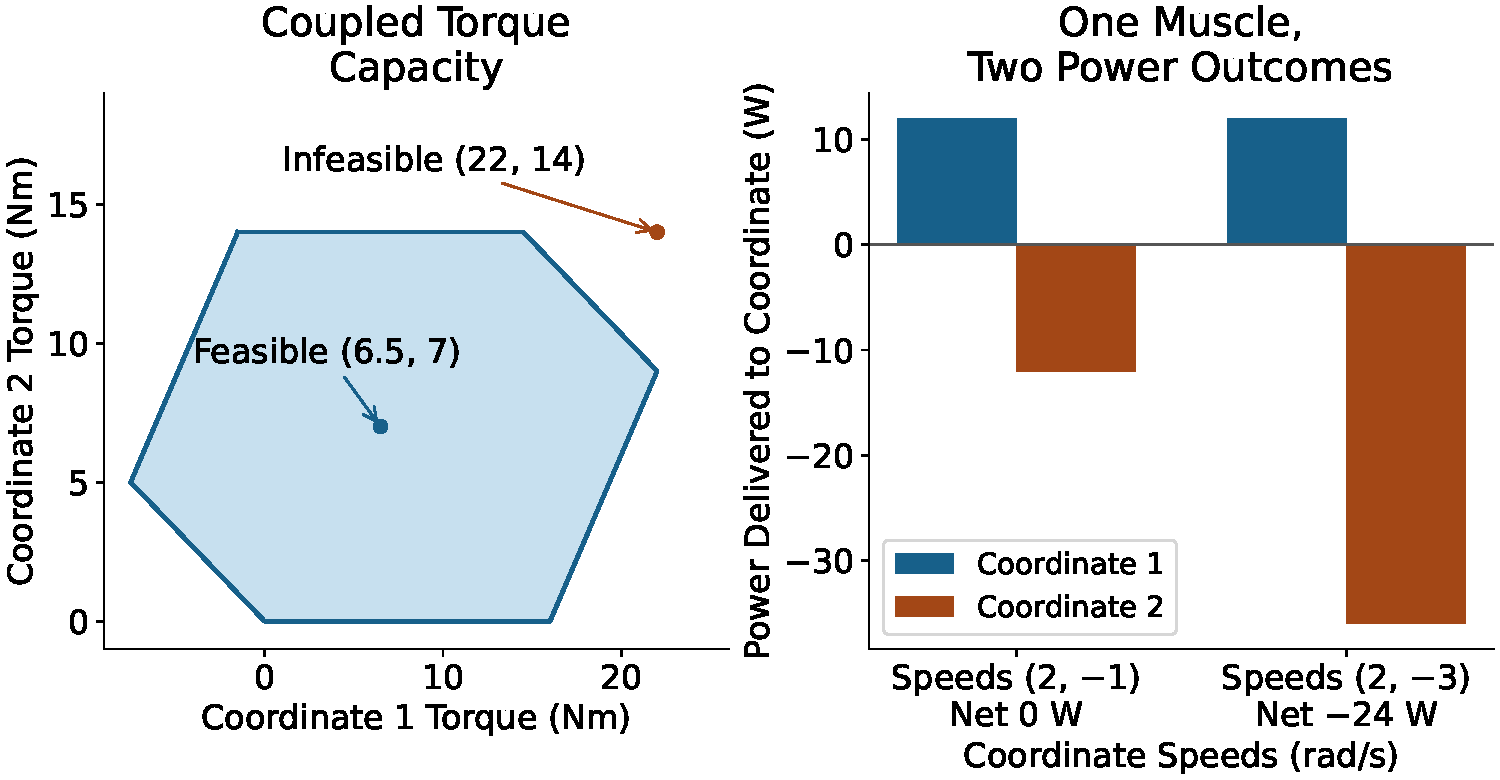
\includegraphics[width=\linewidth]{figures/muscle_torque_feasibility.pdf}
\caption{The Feasible Torque Set and Signed Joint Powers}
\label{fig:muscle-jacobian}
\end{figure}

\begin{definition}{Co-Contraction}{cocontraction}
Co-contraction is simultaneous activity of muscles with opposing torque effects about a specified coordinate. A null-space perturbation is not necessarily co-contraction: it can redistribute force between synergists. Conversely, changing antagonist activity need not preserve net torque. State the muscles, coordinate, baseline forces and compensation when interpreting a recruitment change.
\end{definition}

\subsection{Why Redundancy Matters for Golf}

The same net torque can be associated with different internal forces, contact loads, activation costs and responses to perturbations. This makes muscle sharing important when studying tissue loading or robustness. It does not show that more co-contraction is always useful, or that a golfer should maximize stiffness at impact. Those are task-specific claims requiring a model of the relevant disturbance, contact and time interval.

To see why stiffness requires a separate calculation, consider fixed internal states and conservative path tension $F_j(\ell_j)$. Let $U=\sum_j U_j(\ell_j)$ with $dU_j/d\ell_j=F_j$. Since $\bm\tau_M=-\nabla_qU$, define restoring tangent stiffness as $\bm K_q=-\partial\bm\tau_M/\partial\bm q$. Then
\[
\bm K_q=\bm L^T\bm K_\ell\bm L+
\sum_j F_j\nabla_q^2\ell_j,\qquad
\bm K_\ell=\operatorname{diag}(dF_j/d\ell_j).
\]
The first term reflects material stiffness; the second reflects geometry under tension. A positive first term does not ensure a positive sum. With nonconservative or feedback-controlled muscles, use the appropriate state-dependent linearization instead of assuming an energy Hessian.

For a concrete counterexample, attach a spring from a fixed anchor $a=0.1$ m from a pivot to a point rotating at radius $b=0.2$ m. Its length is $\ell(q)=\sqrt{a^2+b^2-2ab\cos q}$. With stiffness $k=1000$ N/m and slack length $0.2$ m, the spring is taut at $q=\pi$: $\ell=0.3$ m and $F=100$ N. There $\ell'=0$ and $\ell''=-ab/(a+b)$, so
\[
K_q=k(\ell')^2+F\ell''=-20/3\ {\rm Nm/rad}.
\]
The equilibrium is an energy maximum despite positive spring stiffness. Finite differences of spring energy verify the negative curvature. This is a mechanics counterexample, not a quantitative wrist model. Positive restoring stiffness is itself distinct from asymptotic stability, which also depends on inertia, damping, other states, constraints and feedback. Undamped oscillations do not decay merely because stiffness is positive.

\subsection{In the Control-Affine Framework}

A joint-torque input replaces detailed recruitment by its aggregate generalized-force effect. It is useful for a declared rigid-body question, but hides the feasible force set and internal states unless they are explicitly restored. In general, the controls in $\dot{\bm x}=f(\bm x)+G(\bm x)\bm u$ need not be joint torques. They may be motor currents, muscle excitations or other inputs if the chosen state equations have the required dependence on them. An activation model that is affine in excitation can still have nonlinear force generation downstream.

\begin{laymansbox}{What the Torque Description Leaves Open}{box:redundancy-black-box}
Two force patterns can provide the same turning effect while loading the body differently. A torque-based result can identify a useful mechanical demand. The muscle model must still show how that demand can be produced and what the internal consequences are.
\end{laymansbox}

\section{Joint Torques as a Modeling Choice}
\label{sec:why-joint-torques}

A constrained whole-body model can be written in generalized-speed coordinates as
\[
\dot{\bm q}=\bm N(\bm q)\bm v,\qquad
\bm M(\bm q)\dot{\bm v}+\bm h(\bm q,\bm v)
=\bm B\bm u+\bm Q_{\rm passive}
+\bm Q_{\rm known}+\bm J_v^T\bm\lambda.
\]
Here $\bm h$ includes modeled inertial velocity terms and gravity; $\bm B$ maps actuator inputs to forces conjugate to $\bm v$; and $\bm J_v$ maps $\bm v$ to the contact velocity components conjugate to $\bm\lambda$. Contact reactions must satisfy the declared contact equations and inequalities. If a coordinate-rate Jacobian $\bm J_c$ instead maps $\dot{\bm q}$ to those same velocity components, then $\bm J_v=\bm J_c\bm N$. Thus $\bm J_v^T\bm\lambda=\bm N^T\bm J_c^T\bm\lambda$ preserves contact power. In a muscle-driven model, replace the actuator term by $-\bm N^T\bm L^T\bm F$ together with the muscle state equations. A floating base has unactuated directions; it cannot be assigned arbitrary independent joint-torque controls.

\subsection{Sufficiency}

For fixed inertial and geometric parameters, complete initial conditions, specified external forces and a well-posed contact mode, the same total generalized forces give the same instantaneous rigid-body acceleration. The same complete force histories then give the same motion when the initial-value problem has a unique solution. This is a conditional equivalence, not proof that torques alone predict every aspect of the human body. A change in contact mode, compliance or internal actuator state can invalidate the reduced description or alter its future inputs.

\subsection{Redundancy Avoidance}

Torque-driven optimization can study mechanical coordination without first selecting individual muscle forces. The cost is an omitted recruitment problem. An unconstrained torque trajectory may be impossible to realize with tensile actuators, especially with biarticular coupling, delays or state-dependent capacity. A useful workflow first identifies a mechanical opportunity, then asks whether a muscle-driven model can realize it under the same task and boundary conditions. Agreement must be checked rather than assumed.

\subsection{Experimental Accessibility}

Motion capture supplies observations from which kinematics are estimated; force plates measure contact forces and moments over their instrumented surfaces. Inverse dynamics combines such data with inertial parameters, coordinate definitions and a contact model to estimate net generalized forces. It does not directly measure every joint torque or uniquely identify individual muscle tensions. Unmeasured hand-club forces, filtering, differentiation, segment parameters and multiple contacts can affect the result.

A dynamometer measures an external force or moment under specified test conditions. Surface electromyography measures electrical activity associated with muscle excitation; it is neither an invasive force transducer nor a direct measure of tendon tension. EMG-informed force estimates require additional assumptions about activation, geometry and contraction dynamics. Even accurate net-moment agreement cannot identify all muscle forces when the map has a null space.

The upper-extremity model of Holzbaur and colleagues illustrates both the value and limits of such models. Its geometry and muscle parameters support specific comparisons, and some parameters were adjusted against joint-moment data. Those fitted comparisons should be distinguished from other validation tasks. Prescribed scapular motion, generic geometry and omitted intrinsic hand muscles limit transfer to golf-grip questions. \citep{Holzbaur2005}

\subsection{Connection to Control}

Solving a fixed-contact rigid-body system for acceleration can produce affine dependence on applied torque when the dynamics and constraint equations are linear in those inputs. This does not ensure a globally affine model through contact switching, friction transitions or muscle-state changes. The model must specify the chosen inputs and operating domain. A coordinate's generalized force is power-conjugate to its speed; it need not be an independently selectable control. Translational coordinates have conjugate forces in newtons, rather than rotational torques in newton-metres.

\begin{principle}{What a Torque Model Establishes}{prin:why-joint-torques}
A declared torque-driven model can explain how aggregate inputs influence motion and impact conditions. Feasibility, recruitment, muscle energy, internal load and perturbation response require additional information. A mechanically successful solution becomes a physiological hypothesis only after those missing constraints and observations are addressed.
\end{principle}

\subsection{What Is Lost?}

A net torque history does not specify opposing muscle forces, tendon energy, metabolic expenditure, activation reserve or tissue stress. Instantaneous cancellation of opposing torques does not imply relaxed muscles or zero metabolic cost. Conversely, a nonzero torque need not represent active muscle work: passive tissue can contribute. Keep each quantity tied to its own measurement or constitutive model. The chapter on muscle force generation develops the tendon, fiber and activation states needed to make this connection more explicit.

\section{Biarticular Muscles: Coupling Between Joints}
\label{sec:biarticular}

A muscle path can have nonzero moment arms at several coordinates. Biceps brachii spans the shoulder and elbow region and also has a role in forearm rotation. Only the long head of triceps crosses the shoulder; the other heads should not be assigned that same geometry. Wrist flexors and extrinsic finger flexors are different groups: a muscle named for wrist flexion does not thereby cross the finger joints. A model must represent specific heads, attachments and coordinates rather than assign every member of a group identical leverage.

\subsection{The Moment Arm Matrix for Biarticular Muscles}

For muscle $j$, its contribution at coordinate $i$ is $\tau_{ij}=r_{ij}F_j$. Two nonzero entries in the same muscle column of $\bm r$ imply coupled torque contributions. At a fixed configuration their ratio is fixed by geometry when the denominator is nonzero. Coupled torque does not imply equal angular velocities or a prescribed phase order; the entire multibody system determines the motion.

\begin{definition}{Biarticular Coupling}{biarticular}
One tensile path can exert torques at several joints. Their signs and magnitudes follow its moment arms; their instantaneous powers also require the respective coordinate velocities. Anatomical coupling alone establishes neither the direction of energy transfer nor a universal proximal-to-distal sequence.
\end{definition}

\subsection{Energy Transfer via Biarticular Muscles}

For the configuration-only workless path,
\[
P_{ij}=r_{ij}F_j\dot q_i,\qquad
\sum_iP_{ij}=-F_j\dot\ell_j.
\]
Positive $P_{ij}$ denotes mechanical power delivered to that coordinate by the muscle path; negative power denotes absorption from it. For the second muscle of the two-joint example, $\bm r_j=(0.02,0.04)^T$ m and $F_j=300$ N. At speeds $(2,-1)^T$ rad/s, the powers are $(12,-12)^T$ W. The path absorbs power at coordinate 2 and delivers it at coordinate 1, with zero net path power at that instant. The direction reverses if both velocities reverse. Calling this automatically proximal-to-distal would be incorrect.

At speeds $(2,-3)^T$ rad/s, the same torque contributions instead produce $(12,-36)^T$ W and net absorption of $24$ W. Positive powers at both joints would indicate net generation. Thus a path can transmit, generate or absorb mechanical power depending on its state and motion. Joint-coordinate power partitions are representation-dependent; their sum must preserve total work under a consistent coordinate transformation.

Zero total path power does not imply zero fiber power or zero metabolic expenditure. A compliant tendon can exchange stored energy with shortening or lengthening fibers while total muscle-tendon length stays instantaneously fixed. Include tendon energy and the fiber constitutive model before attributing the power to active contraction, elastic return or dissipation. Segment-level energy transfer also requires a consistent segment force-and-moment power balance; a sequence of joint-speed peaks is not that balance.

\begin{laymansbox}{Reading the Direction of Power}{box:biarticular-energy}
A connection between two joints is like a transmission whose direction of power flow depends on how it is loaded and moving. Knowing that the connection exists is only the beginning. Measure or model force and motion together before deciding which side supplies power and which receives it.
\end{laymansbox}

\subsection{Example: The Wrist Flexors in Golf}

Wrist flexion-extension, radial-ulnar deviation and forearm pronation-supination are different coordinates. Their axes also differ from the club shaft axis. A muscle's contribution to club rotation therefore depends on anatomical posture, the hand-club contact geometry and the rest of the body. It cannot be deduced by relabeling wrist flexion as shaft roll. The upper-extremity modeling literature provides specific muscle paths and coordinate definitions, but a generic arm model is not a validated model of a two-handed golf grip. \citep{Holzbaur2005}

\section[The Inverse Problem: From Desired Torques to Muscle Forces]{The Inverse Problem:\\From Desired Torques to Muscle Forces}
\label{sec:inverse-problem}

\subsection{The Underdetermined Inverse}

Suppose inverse dynamics supplies a net generalized-force estimate and modeled passive and other contributions have been separated consistently. The remaining muscle demand is $\bm\tau_M^*$. Solving $\bm r\bm F=\bm\tau_M^*$ first requires a feasible target. Being in the column space of $\bm r$ is necessary for an unconstrained real solution, but insufficient for nonnegative capacity-bounded tension. A pseudoinverse can return negative muscle forces. A feasible target can also have multiple force realizations, each with different internal consequences.

The illustrative set $\bm0\leq\bm F\leq\overline{\bm F}$ should not be read as instantaneous voluntary access to every force in that box. With tendon compliance, the current tendon state constrains tension; excitation changes subsequent activation and contraction. Passive tension can also set a nonzero lower bound. The reachable force set depends on state and time horizon. A sequence of feasible static snapshots can fail to form one dynamically realizable muscle trajectory.

\subsection{Optimization Approaches}

One explicit static criterion is normalized squared force:
\[
\min_{\bm F}\sum_j(F_j/\overline F_j)^2
\quad\hbox{subject to}\quad
\bm r\bm F=\bm\tau_M^*,\quad
\bm0\leq\bm F\leq\overline{\bm F}.
\]
With positive capacities and a nonempty convex feasible set, this strictly convex objective has a unique minimizing force vector. Uniqueness follows from the stated mathematical criterion, not from evidence that the nervous system uses it. An unnormalized sum of squared forces is a different criterion and weights muscle capacities differently. Neither is automatically metabolic energy.

An energy or fatigue objective requires a specified constitutive model with the appropriate states and units. A trajectory optimization may include activation dynamics, force-length-velocity behavior, tendon energy and history-dependent fatigue. Its result is conditional on those equations, parameter choices, boundary conditions and objective. Comparing alternative plausible objectives and checking sensitivity is more informative than presenting a single optimizer output as identified human recruitment.

\begin{definition}{Static Optimization}{static-opt}
Static optimization solves a force-sharing problem at each sampled instant using declared constraints and a criterion. Some formulations include state-dependent force capacities, but separate instantaneous problems do not by themselves enforce a consistent activation or tendon trajectory. They can estimate recruitment under assumptions; they do not establish the brain's algorithm.
\end{definition}

\subsection{Why This Matters for Golf (And Why It Is Hard)}

An observed swing and its net torques can constrain hypotheses without identifying one muscle strategy. EMG, imaging, perturbation responses and contact measurements add different information, each with its own limitations. A stronger study calibrates model parameters on designated data, checks predictions on separate conditions, and reports sensitivity to measurement and model uncertainty. Good net-moment fit alone cannot remove a null space in the muscle-force map.

\begin{laymansbox}{From a Swing Outcome to a Testable Hypothesis}{box:inverse-problem-golf}
A player reaches a given clubhead speed. One proposed change uses a different muscle pattern to obtain the same speed with lower cost. To assess it, specify the complete task, the force and contact constraints, the cost model and the observations that could distinguish the patterns. The common clubhead speed establishes the shared outcome; it does not establish the proposed recruitment or its benefit.
\end{laymansbox}

\section{Practical Example: The Golf Grip}
\label{sec:grip-forces}

\subsection{Anatomy of the Grip}

Finger flexors, finger extensors, wrist muscles and intrinsic hand muscles contribute different actions. Their anatomical paths determine joint torques, while the contact distribution between hand and handle determines the wrench applied to the club. A count of a few named muscles cannot replace a complete model of the fingers, thumb, palm and forearm. For the present discussion, the contact equations clarify what must be connected without pretending to supply a personalized recruitment model.

\subsection{Grip Force vs. Grip Torque}

Represent hand contact by patches $k$ at positions $\bm\rho_k$ relative to a declared club reference point. With patch forces $\bm f_k$ and any modeled patch couples $\bm m_k$, the applied wrench is
\[
\bm f_{\rm hand}=\sum_k\bm f_k,\qquad
\bm m_{\rm hand}=\sum_k(\bm\rho_k\times\bm f_k+\bm m_k).
\]
A normal compressive load and a net wrench are different summaries of that distribution. Opposing normal forces can largely cancel in the net force while increasing pressure and friction capacity. Under a simple Coulomb patch model, tangential force is limited by $\|\bm f_{t,k}\|\leq\mu_k f_{n,k}$ with $f_{n,k}\geq0$. This is a declared contact approximation, not an established constant friction coefficient for every hand, glove and grip. Contact deformation and torsional resistance require further modeling.

If $\bm v_c=\bm J_c\dot{\bm q}$ maps skeletal motion to a contact-point velocity, $\bm J_c^T\bm f_c$ maps the force acting on the skeleton to generalized force. When $\dot{\bm q}=\bm N\bm v$, the speed-coordinate force is $\bm N^T\bm J_c^T\bm f_c$. Include the angular-velocity Jacobian when retaining contact couples. Force on the club has the opposite sign at the same interface. The same work-conjugacy discipline used for muscle tension prevents a hidden sign error here. A measured pressure map or net wrench does not uniquely identify all muscle forces.

\subsection{Moment Arm Changes With Hand Configuration}

A strong or weak grip describes a hand-club arrangement, not a single specified wrist angle or muscle moment arm. A grip change can alter anatomical posture, contact locations and club orientation in different combinations. Predicting the change requires those configurations and a muscle/contact model. There is no basis in this chapter for universally assigning improved leverage to flexor carpi ulnaris in a strong grip or flexor carpi radialis in a weak grip.

The useful modeling question is conditional: at the measured posture, how do feasible wrist and finger forces project through the contact geometry into the desired club wrench? Then ask whether a changed posture alters contact retention, available torque, comfort or repeatability under the same task. Geometry may suggest a hypothesis; it does not establish a coaching prescription.

\subsection{Grip Force Modulation During the Swing}

Grip loading can vary with motion, club inertia and interaction forces. To quantify its time history, identify the sensor, measured quantity, calibration, temporal resolution and normalization. Instrumented handles or pressure sensors supply information that a ground force plate cannot directly provide. Surface EMG requires an additional force-estimation model. A percentage of maximum is uninterpretable without the reference test, posture and measured quantity.

Accordingly, this chapter does not assign universal grip-force percentages to backswing, transition, downswing or impact. An experimentally supported account would report the actual study population, task and uncertainty. The absence of such evidence does not mean grip force is constant; it means a particular numerical pattern has not been established here.

\subsection{Grip Stiffness and Impact}

Clubhead-ball contact force is not identical to force transmitted to the hands. The shaft's distributed inertia and compliance, contact duration, grip conditions and pre-impact state govern that transmission. A large clubhead force alone cannot establish an optimal wrist stiffness. Nor does a brief collision imply that an arbitrary new neural command can generate a useful muscle-force change within the remaining interval.

Distinguish pre-existing muscle activation and mechanical impedance from later feedback responses. A defensible impact hypothesis specifies the coupled hand-club-ball model, perturbation, time horizon and performance outcome. It then compares feasible preparations or interventions from matched initial states. Increased co-contraction may change load and impedance, but its effect on face orientation, speed or variability must be evaluated. The goal is to explain which mechanisms matter under which conditions, rather than turn an unspecified impact-force estimate into a universal instruction to grip harder.

\begin{principle}{Key Takeaways}{prin:muscle-torque-takeaways}
Muscle geometry, force generation, contact mechanics and control are linked through work and state-dependent constraints. With positive tension and positive lengthening, $\bm\tau_M=-\bm L^T\bm F$. Torque feasibility requires bounds and dynamics, not only a matrix inverse. Biarticular powers require velocities as well as moment arms. Net torque does not uniquely determine recruitment, stiffness, energy or tissue load. A golf hypothesis becomes stronger when its proposed causal chain is explicit and each link has an appropriate calculation or observation.
\end{principle}

\begin{exercises}{Chapter Exercises}{ex:muscle-torque-exercises}
\begin{enumerate}
\item Define a signed axial moment arm. Explain when a perpendicular distance is sufficient, and derive the sign of $\bm\tau_M=-\bm L^T\bm F$ from tensile virtual work.

\item A hypothetical actuator transmits 600 N at moment arms 0.05 m and 0.03 m. Compute both torque contributions. Explain why this does not locate a person's maximum-strength posture.

\item For the nonsymmetric two-joint example in this chapter, compute both muscle contributions, the total torque, path rates at speeds $(2,-3)^T$ rad/s and total skeletal power. Explain why transposing the displayed torque map again changes the answer.

% Keep the whole question together at this break in the printed exercise box.
\tcbbreak
\item For the three-muscle feasible-family example, verify the null direction and derive the allowable interval of $t$. Are the independent coordinate maxima simultaneously feasible?

\item Define co-contraction and distinguish it from a null-space force redistribution. Explain how the taut-spring example disproves the claim that positive material stiffness guarantees joint stability.

\item Two synergists have positive moment arms 0.04 m and 0.02 m, each with capacity 1000 N. Characterize all nonnegative force pairs producing 50 Nm. Explain whether this freedom is antagonist co-contraction.

\item State a force-sharing optimization and the assumptions under which its optimum is unique. Explain why that uniqueness does not identify the nervous system's objective or guarantee a dynamically feasible trajectory.

\item Compute the second muscle's joint powers at speeds $(2,-1)^T$ and $(2,-3)^T$ rad/s. Identify the direction of instantaneous transfer in the zero-sum case and explain what remains unknown about tendon and metabolic energy.

\item Design the measurements needed to support a phase-dependent grip-force claim. Distinguish handle pressure, net wrench, ground reaction and surface EMG.

\item Explain why changing from a strong to a weak grip does not specify a unique change in the wrist moment-arm matrix. Identify the anatomical and contact information required for a prediction.

\item For the constraint $\bm q=(s,2s)^T$, compute the reduced torque in the two-joint example. Explain why a torque-input model also needs actuator feasibility and appropriate floating-base/contact equations.
\end{enumerate}
\end{exercises}

\section{Worked Answers and Modeling Checks}

\begin{enumerate}
\item $r_e=\bm e\cdot(\bm\rho\times\bm d)$. Its planar magnitude reduces to the pivot-to-force-line distance. With $\delta W=-\bm F^T\bm L\delta\bm q$, matching the coefficient of independent $\delta\bm q$ gives $\bm\tau_M=-\bm L^T\bm F$. Axis orientation and tension convention must be stated.

\item The contributions are 30 Nm and 18 Nm. The assumed tension is held equal; a person's attainable tension need not be equal at the two postures. No angle, force-length state or measured capacity has been supplied.

\item The contributions are $(25,0)^T$ and $(6,12)^T$ Nm, totaling $(31,12)^T$ Nm. Path rates are $(-0.10,0.08)^T$ m/s and total power is 26 W. Multiplying $\bm r^T\bm F$ would instead give $(25,22)^T$ for these equal-sized matrices and mismatched row meanings; it is not the declared force map.

\item $\bm r(13,-8,12)^T=\bm0$. The force inequalities give $t\in[-25/6,50/3]$ N. Coordinate maxima 22 and 14 Nm cannot coexist: the force choice required for 14 Nm at coordinate 2 leaves at most 14.5 Nm at coordinate 1.

\item Co-contraction concerns opposing actions about a named coordinate; a null direction can instead exchange synergist forces. At the taut-spring equilibrium, the material contribution vanishes because $\ell'=0$ and the geometric contribution is $F\ell''=-20/3$ Nm/rad. The equilibrium is an energy maximum. Even a positive restoring stiffness would not alone establish asymptotic stability without the remaining dynamics.

\item $F_2=2500\,{\rm N}-2F_1$, with $750\,{\rm N}\leq F_1\leq1000\,{\rm N}$ and correspondingly $500\,{\rm N}\leq F_2\leq1000\,{\rm N}$. This is a continuum of feasible synergist sharing, not an antagonist pair. A demand above 60 Nm would be infeasible under these bounds; at 60 Nm both forces must be at capacity.

\item Positive-capacity normalized squared force is strictly convex, so a nonempty convex bounded feasible set has one minimizer. Changing the criterion changes the inference. Independent samples do not enforce activation or tendon dynamics; a neural interpretation requires additional evidence.

\item Powers are $(12,-12)^T$ W and $(12,-36)^T$ W. In the first case, power is absorbed at coordinate 2 and delivered at coordinate 1; in the second, net path power is $-24$ W. Fiber work, tendon storage and metabolic cost remain separate quantities.

\item Use calibrated instrumented-handle or pressure measurements synchronized with kinematics and a defined phase convention. Specify whether the result is contact pressure, integrated normal load or a full wrench, and define the normalization test. Ground forces and EMG are complementary observations, not substitutes for direct handle-force measurement.

\item Measure posture and hand-club placement, define joint and shaft axes, specify muscle paths and a contact model, and propagate their uncertainty. The verbal grip category alone does not supply these quantities or identify a universally advantaged muscle.

\item The reduced torque is $31+2(12)=55$ Nm, with effective moment arms $(0.05,0.10)$ m. This preserves virtual work along the allowed coordinate motion. It does not make the underlying tensions freely controllable or eliminate unactuated base directions, contact feasibility or actuator state dynamics.
\end{enumerate}

The nine independent checks in the accompanying verification module reproduce the geometry, transpose, power, feasible-force, coupled-coordinate, integrability and stiffness examples. They test these constructed derivations. Empirical claims about a particular golfer still require suitable observations and model validation.
\clearpage
\flushbottom{}
